\documentclass[10pt]{beamer}
\usepackage[utf8]{inputenc}
\usepackage{tikz, pgfplots}
\pgfplotsset{compat=1.18}
\usetikzlibrary{positioning}
\usetikzlibrary{trees}
\usetikzlibrary{shapes.geometric, arrows.meta, positioning}
\usepackage{xcolor}
\usetheme{EastLansing}
\usepackage{graphicx}
\usepackage{subcaption}
\usepackage{hyperref} 
\usepackage{colortbl} % Required for \rowcolor
\usepackage{animate}
\usepackage[T1]{fontenc}
\usepackage{amsmath, amsfonts, amssymb}
\usepackage[french]{babel}
\usepackage[normalem]{ulem}
\setbeamertemplate{caption}[numbered]
\usepackage{multirow}
\title{Rapport Hebdo}
\author{Viet Anh Quach}
\institute{3SR}
\date{\today}

\begin{document}

\begin{frame}
    \titlepage
\end{frame}


\section{DEM}
\begin{frame}{Changer le modèle}
    \begin{figure}[h]
        \centering
        \scalebox{0.15}{\includegraphics{rentangulaire.png}}
        \caption{Boîte rentangulaire}
    \end{figure}
\end{frame}


\begin{frame}{Étude sur le nombre d'inertie}
    \begin{table}
        \centering
        \begin{tabular}{|c|c|c|c|}
            \hline
            \textbf{Symboles}               & \textbf{Paramètres} & \textbf{Valeurs}                      & \textbf{Unité}  \\
            \hline
            Nombre de particules            & N                   & $15 \times 30 \times 15 = 6750$       & -               \\
            \hline
            Le rayon des particules         & R                   & 0.003 $\div$ 0.005                    & m               \\
            \hline
            Masse volumique                 & $\rho$              & 2500                                  & $\text{kg/m}^3$ \\
            \hline
            Raideur normale et tangentielle & $k_n$ \& $k_t$      & \textcolor{black}{$3 \times 10^6$}    & $\text{N/m}$    \\
            \hline
            Niveau de raideur               & $\kappa$            & >1000                                 & -               \\
            \hline
            Coefficient de frottement       & $\mu$               & $\mu_{iso} = 0.1, \mu_{triax} = 0.5 $ & -               \\
            \hline
            Coefficient d'amortissement     & $\alpha$            & 0.0                                   & -               \\
            \hline
        \end{tabular}
        \caption{Valeurs gardé}
    \end{table}
\end{frame}


\begin{frame}{Étude sur le nombre d'inertie}
    \begin{columns}
        \begin{column}{0.5\textwidth}
            \begin{table}
                \centering
                \begin{tabular}{|c|c|c|c|}
                    \hline
                    % \textbf{v (m/s) \&P (kPa)} & $3 \times 10^4$ & $3 \times 10^2$                       & $3 \times 10^0$ & $3 \times 10^{-2}$ & $3 \times 10^{-4}$ \\
                    $v $(m/s)                & $ \sigma_3 = 3 \times 10^2$ (kPa) \\
                    \hline
                    $4.542   \times 10^{-3}$ & I = $10^{-5}$                     \\
                    \hline
                    $4.542   \times 10^{-2}$ & I = $10^{-4}$                     \\
                    \hline
                    $4.542   \times 10^{-1}$ & I = $10^{-3}$                     \\
                    \hline
                    $4.542   \times 10^{0}$  & I = $10^{-2}$                     \\
                    \hline
                    $4.542   \times 10^{1}$  & I = $10^{-1}$                     \\
                    \hline
                    $4.542   \times 10^{2}$  & I = $1$                           \\
                    \hline
                \end{tabular}
                \caption{Changer la vitess}
            \end{table}
        \end{column}
        \begin{column}{0.5\textwidth}
            \begin{table}
                \centering
                \begin{tabular}{|c|c|c|c|}
                    \hline
                    % \textbf{v (m/s) \&P (kPa)} & $3 \times 10^4$ & $3 \times 10^2$                       & $3 \times 10^0$ & $3 \times 10^{-2}$ & $3 \times 10^{-4}$ \\
                    $\sigma_{3} $(kPa) & v $ = 4.542   \times 10^{-2}$ (m/s) \\
                    \hline
                    $3 \times 10^4$    & I = $10^{-5}$                       \\
                    \hline
                    $3 \times 10^2$    & I = $10^{-4}$                       \\
                    \hline
                    $3 \times 10^0$    & I = $10^{-3}$                       \\
                    \hline
                    $3 \times 10^{-2}$ & I = $10^{-2}$                       \\
                    \hline
                    $3 \times 10^{-4}$ & I = $10^{-1}$                       \\
                    \hline
                    $3 \times 10^{-7}$ & I = $1$                             \\
                    \hline
                \end{tabular}
                \caption{Changer la contrainte de confinement}
            \end{table}
        \end{column}
    \end{columns}
\end{frame}

\begin{frame}{Changer la contrainte}
    \begin{columns}
        \begin{column}{0.5\textwidth}
            \begin{figure}[h]
                \centering
                \scalebox{0.5}{% GNUPLOT: LaTeX picture with Postscript
\begingroup
  \makeatletter
  \providecommand\color[2][]{%
    \GenericError{(gnuplot) \space\space\space\@spaces}{%
      Package color not loaded in conjunction with
      terminal option `colourtext'%
    }{See the gnuplot documentation for explanation.%
    }{Either use 'blacktext' in gnuplot or load the package
      color.sty in LaTeX.}%
    \renewcommand\color[2][]{}%
  }%
  \providecommand\includegraphics[2][]{%
    \GenericError{(gnuplot) \space\space\space\@spaces}{%
      Package graphicx or graphics not loaded%
    }{See the gnuplot documentation for explanation.%
    }{The gnuplot epslatex terminal needs graphicx.sty or graphics.sty.}%
    \renewcommand\includegraphics[2][]{}%
  }%
  \providecommand\rotatebox[2]{#2}%
  \@ifundefined{ifGPcolor}{%
    \newif\ifGPcolor
    \GPcolortrue
  }{}%
  \@ifundefined{ifGPblacktext}{%
    \newif\ifGPblacktext
    \GPblacktextfalse
  }{}%
  % define a \g@addto@macro without @ in the name:
  \let\gplgaddtomacro\g@addto@macro
  % define empty templates for all commands taking text:
  \gdef\gplbacktext{}%
  \gdef\gplfronttext{}%
  \makeatother
  \ifGPblacktext
    % no textcolor at all
    \def\colorrgb#1{}%
    \def\colorgray#1{}%
  \else
    % gray or color?
    \ifGPcolor
      \def\colorrgb#1{\color[rgb]{#1}}%
      \def\colorgray#1{\color[gray]{#1}}%
      \expandafter\def\csname LTw\endcsname{\color{white}}%
      \expandafter\def\csname LTb\endcsname{\color{black}}%
      \expandafter\def\csname LTa\endcsname{\color{black}}%
      \expandafter\def\csname LT0\endcsname{\color[rgb]{1,0,0}}%
      \expandafter\def\csname LT1\endcsname{\color[rgb]{0,1,0}}%
      \expandafter\def\csname LT2\endcsname{\color[rgb]{0,0,1}}%
      \expandafter\def\csname LT3\endcsname{\color[rgb]{1,0,1}}%
      \expandafter\def\csname LT4\endcsname{\color[rgb]{0,1,1}}%
      \expandafter\def\csname LT5\endcsname{\color[rgb]{1,1,0}}%
      \expandafter\def\csname LT6\endcsname{\color[rgb]{0,0,0}}%
      \expandafter\def\csname LT7\endcsname{\color[rgb]{1,0.3,0}}%
      \expandafter\def\csname LT8\endcsname{\color[rgb]{0.5,0.5,0.5}}%
    \else
      % gray
      \def\colorrgb#1{\color{black}}%
      \def\colorgray#1{\color[gray]{#1}}%
      \expandafter\def\csname LTw\endcsname{\color{white}}%
      \expandafter\def\csname LTb\endcsname{\color{black}}%
      \expandafter\def\csname LTa\endcsname{\color{black}}%
      \expandafter\def\csname LT0\endcsname{\color{black}}%
      \expandafter\def\csname LT1\endcsname{\color{black}}%
      \expandafter\def\csname LT2\endcsname{\color{black}}%
      \expandafter\def\csname LT3\endcsname{\color{black}}%
      \expandafter\def\csname LT4\endcsname{\color{black}}%
      \expandafter\def\csname LT5\endcsname{\color{black}}%
      \expandafter\def\csname LT6\endcsname{\color{black}}%
      \expandafter\def\csname LT7\endcsname{\color{black}}%
      \expandafter\def\csname LT8\endcsname{\color{black}}%
    \fi
  \fi
    \setlength{\unitlength}{0.0500bp}%
    \ifx\gptboxheight\undefined%
      \newlength{\gptboxheight}%
      \newlength{\gptboxwidth}%
      \newsavebox{\gptboxtext}%
    \fi%
    \setlength{\fboxrule}{0.5pt}%
    \setlength{\fboxsep}{1pt}%
    \definecolor{tbcol}{rgb}{1,1,1}%
\begin{picture}(7200.00,5040.00)%
    \gplgaddtomacro\gplbacktext{%
      \csname LTb\endcsname%%
      \put(1210,1144){\makebox(0,0)[r]{\strut{}$0$}}%
      \csname LTb\endcsname%%
      \put(1210,1512){\makebox(0,0)[r]{\strut{}$0.0002$}}%
      \csname LTb\endcsname%%
      \put(1210,1879){\makebox(0,0)[r]{\strut{}$0.0004$}}%
      \csname LTb\endcsname%%
      \put(1210,2247){\makebox(0,0)[r]{\strut{}$0.0006$}}%
      \csname LTb\endcsname%%
      \put(1210,2614){\makebox(0,0)[r]{\strut{}$0.0008$}}%
      \csname LTb\endcsname%%
      \put(1210,2982){\makebox(0,0)[r]{\strut{}$0.001$}}%
      \csname LTb\endcsname%%
      \put(1210,3349){\makebox(0,0)[r]{\strut{}$0.0012$}}%
      \csname LTb\endcsname%%
      \put(1210,3717){\makebox(0,0)[r]{\strut{}$0.0014$}}%
      \csname LTb\endcsname%%
      \put(1210,4084){\makebox(0,0)[r]{\strut{}$0.0016$}}%
      \csname LTb\endcsname%%
      \put(1210,4452){\makebox(0,0)[r]{\strut{}$0.0018$}}%
      \csname LTb\endcsname%%
      \put(1210,4819){\makebox(0,0)[r]{\strut{}$0.002$}}%
      \csname LTb\endcsname%%
      \put(1342,924){\makebox(0,0){\strut{}$0$}}%
      \csname LTb\endcsname%%
      \put(1978,924){\makebox(0,0){\strut{}$10$}}%
      \csname LTb\endcsname%%
      \put(2613,924){\makebox(0,0){\strut{}$20$}}%
      \csname LTb\endcsname%%
      \put(3249,924){\makebox(0,0){\strut{}$30$}}%
      \csname LTb\endcsname%%
      \put(3884,924){\makebox(0,0){\strut{}$40$}}%
      \csname LTb\endcsname%%
      \put(4520,924){\makebox(0,0){\strut{}$50$}}%
      \csname LTb\endcsname%%
      \put(5155,924){\makebox(0,0){\strut{}$60$}}%
      \csname LTb\endcsname%%
      \put(5791,924){\makebox(0,0){\strut{}$70$}}%
      \put(5923,1144){\makebox(0,0)[l]{\strut{}$-0.5$}}%
      \put(5923,1512){\makebox(0,0)[l]{\strut{}$0$}}%
      \put(5923,1879){\makebox(0,0)[l]{\strut{}$0.5$}}%
      \put(5923,2247){\makebox(0,0)[l]{\strut{}$1$}}%
      \put(5923,2614){\makebox(0,0)[l]{\strut{}$1.5$}}%
      \put(5923,2982){\makebox(0,0)[l]{\strut{}$2$}}%
      \put(5923,3349){\makebox(0,0)[l]{\strut{}$2.5$}}%
      \put(5923,3717){\makebox(0,0)[l]{\strut{}$3$}}%
      \put(5923,4084){\makebox(0,0)[l]{\strut{}$3.5$}}%
      \put(5923,4452){\makebox(0,0)[l]{\strut{}$4$}}%
      \put(5923,4819){\makebox(0,0)[l]{\strut{}$4.5$}}%
    }%
    \gplgaddtomacro\gplfronttext{%
      \csname LTb\endcsname%%
      \put(341,2981){\rotatebox{-270}{\makebox(0,0){\strut{}q (kPa)}}}%
      \put(6693,2981){\rotatebox{-270}{\makebox(0,0){\strut{}$\varepsilon_v$ (\%)}}}%
      \put(3566,594){\makebox(0,0){\strut{}$\varepsilon_{yy}$ (\%)}}%
      \csname LTb\endcsname%%
      \put(2711,393){\makebox(0,0)[r]{\strut{}$\sigma_3 = 3 \times 10^{-2}$ kPa}}%
      \csname LTb\endcsname%%
      \put(2711,173){\makebox(0,0)[r]{\strut{}$\sigma_3 = 3 \times 10^{0}$ kPa}}%
      \csname LTb\endcsname%%
      \put(5810,393){\makebox(0,0)[r]{\strut{}$\sigma_3 = 3 \times 10^{2}$ kPa}}%
    }%
    \gplbacktext
    \put(0,0){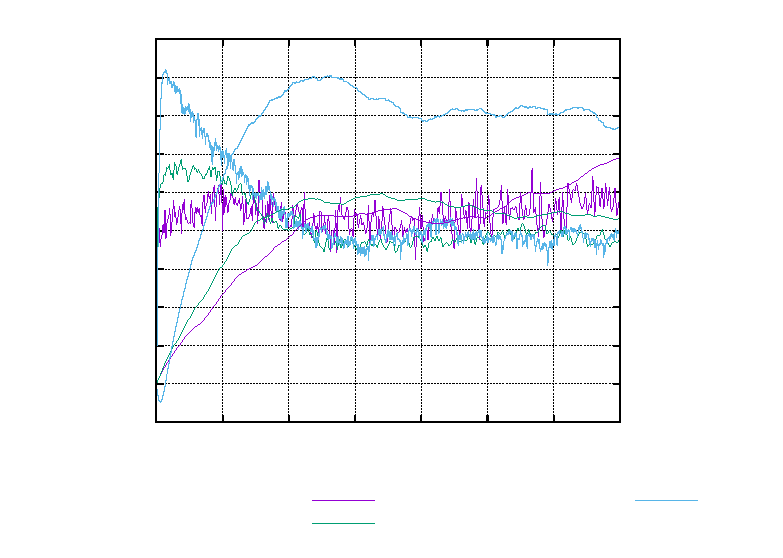
\includegraphics[width={360.00bp},height={252.00bp}]{./Contrainte_contrainteDeviatorique}}%
    \gplfronttext
  \end{picture}%
\endgroup
}
                \caption{Contrainte - Déformation DEM (changer la vitess)}
            \end{figure}
        \end{column}
        \begin{column}{0.5\textwidth}
            \begin{table}
                \centering
                \begin{tabular}{|c|c|c|c|}
                    \hline
                    % \textbf{v (m/s) \&P (kPa)} & $3 \times 10^4$ & $3 \times 10^2$                       & $3 \times 10^0$ & $3 \times 10^{-2}$ & $3 \times 10^{-4}$ \\
                    $\sigma_{3} $(kPa)      & v $ = 4.542   \times 10^{-2}$ (m/s)                  \\
                    \hline
                    $3 \times 10^4$         & $\kappa > 1000$                                      \\
                    \hline
                    $3 \times 10^2$         & I = $10^{-4}$                                        \\
                    \hline
                    \rowcolor{white}
                    $3 \times 10^0$         & \multirow{2}{*}{$\tan {\varphi} \approx 90 \degres$} \\
                    \cline{1-1}
                    $3 \times 10^{-2}$      &                                                      \\
                    \hline

                    $4.542   \times 10^{1}$ & \multirow{2}{*}{IsoComp stabilise pas}               \\
                    \cline{1-1}
                    $4.542   \times 10^{2}$ &                                                      \\
                    \hline
                \end{tabular}
                \caption{Changer la contrainte de confinement}
            \end{table}
        \end{column}
    \end{columns}
\end{frame}

\begin{frame}{Changer la vitess}
    \begin{columns}
        \begin{column}{0.5\textwidth}
            \begin{figure}[h]
                \centering
                \scalebox{0.5}{\input{Vitess-contrainteDeviatorique.tex}}
                \caption{Contrainte - Déformation DEM (changer la vitess)}
            \end{figure}
        \end{column}
        \begin{column}{0.5\textwidth}
            \begin{table}
                \centering
                \begin{tabular}{|c|c|c|c|}
                    \hline
                    % \textbf{v (m/s) \&P (kPa)} & $3 \times 10^4$ & $3 \times 10^2$                       & $3 \times 10^0$ & $3 \times 10^{-2}$ & $3 \times 10^{-4}$ \\
                    $v $(m/s)                & $ \sigma_3 = 3 \times 10^2$ (kPa) \\
                    \hline
                    $4.542   \times 10^{-3}$ & I = $10^{-5}$                     \\
                    \hline
                    $4.542   \times 10^{-2}$ & I = $10^{-4}$                     \\
                    \hline
                    $4.542   \times 10^{-1}$ & I = $10^{-3}$                     \\
                    \hline
                    $4.542   \times 10^{0}$  & I = $10^{-2}$                     \\
                    \hline
                    $4.542   \times 10^{1}$  & I = $10^{-1}$                     \\
                    \hline
                    $4.542   \times 10^{2}$  & I = $1$                           \\
                    \hline
                \end{tabular}
                \caption{Changer la vitess}
            \end{table}
        \end{column}
    \end{columns}
\end{frame}

\begin{frame}{Changer la vitess}
    \begin{columns}
        \begin{column}{0.5\textwidth}
            \begin{figure}[h]
                \centering
                \scalebox{0.5}{\input{Vitess-contrainteDeviatorique.tex}}
                \caption{Contrainte - Déformation DEM (changer la vitess)}
            \end{figure}
        \end{column}
        \begin{column}{0.5\textwidth}
            \begin{figure}[h]
                \centering
                \scalebox{0.5}{\input{PasTemps.tex}}
                \caption{Bruyant concernant pas de temps MPM (avant)}
            \end{figure}
        \end{column}
    \end{columns}
    \[
        \dot{x}(t) = \frac{x(t+\varepsilon) - x(t-\varepsilon)}{2\varepsilon}
    \]
    Problème de arrondir?
\end{frame}

\begin{frame}{Comparer entre les formes de boite}
    \begin{columns}
        \begin{column}{0.5\textwidth}
            \begin{figure}[h]
                \centering
                \scalebox{0.5}{\input{contrainteDeviatorique.tex}}
                \caption{Rectangulaire}
            \end{figure}
        \end{column}
        \begin{column}{0.5\textwidth}
            \begin{figure}[h]
                \centering
                \scalebox{0.5}{% GNUPLOT: LaTeX picture with Postscript
\begingroup
  \makeatletter
  \providecommand\color[2][]{%
    \GenericError{(gnuplot) \space\space\space\@spaces}{%
      Package color not loaded in conjunction with
      terminal option `colourtext'%
    }{See the gnuplot documentation for explanation.%
    }{Either use 'blacktext' in gnuplot or load the package
      color.sty in LaTeX.}%
    \renewcommand\color[2][]{}%
  }%
  \providecommand\includegraphics[2][]{%
    \GenericError{(gnuplot) \space\space\space\@spaces}{%
      Package graphicx or graphics not loaded%
    }{See the gnuplot documentation for explanation.%
    }{The gnuplot epslatex terminal needs graphicx.sty or graphics.sty.}%
    \renewcommand\includegraphics[2][]{}%
  }%
  \providecommand\rotatebox[2]{#2}%
  \@ifundefined{ifGPcolor}{%
    \newif\ifGPcolor
    \GPcolortrue
  }{}%
  \@ifundefined{ifGPblacktext}{%
    \newif\ifGPblacktext
    \GPblacktextfalse
  }{}%
  % define a \g@addto@macro without @ in the name:
  \let\gplgaddtomacro\g@addto@macro
  % define empty templates for all commands taking text:
  \gdef\gplbacktext{}%
  \gdef\gplfronttext{}%
  \makeatother
  \ifGPblacktext
    % no textcolor at all
    \def\colorrgb#1{}%
    \def\colorgray#1{}%
  \else
    % gray or color?
    \ifGPcolor
      \def\colorrgb#1{\color[rgb]{#1}}%
      \def\colorgray#1{\color[gray]{#1}}%
      \expandafter\def\csname LTw\endcsname{\color{white}}%
      \expandafter\def\csname LTb\endcsname{\color{black}}%
      \expandafter\def\csname LTa\endcsname{\color{black}}%
      \expandafter\def\csname LT0\endcsname{\color[rgb]{1,0,0}}%
      \expandafter\def\csname LT1\endcsname{\color[rgb]{0,1,0}}%
      \expandafter\def\csname LT2\endcsname{\color[rgb]{0,0,1}}%
      \expandafter\def\csname LT3\endcsname{\color[rgb]{1,0,1}}%
      \expandafter\def\csname LT4\endcsname{\color[rgb]{0,1,1}}%
      \expandafter\def\csname LT5\endcsname{\color[rgb]{1,1,0}}%
      \expandafter\def\csname LT6\endcsname{\color[rgb]{0,0,0}}%
      \expandafter\def\csname LT7\endcsname{\color[rgb]{1,0.3,0}}%
      \expandafter\def\csname LT8\endcsname{\color[rgb]{0.5,0.5,0.5}}%
    \else
      % gray
      \def\colorrgb#1{\color{black}}%
      \def\colorgray#1{\color[gray]{#1}}%
      \expandafter\def\csname LTw\endcsname{\color{white}}%
      \expandafter\def\csname LTb\endcsname{\color{black}}%
      \expandafter\def\csname LTa\endcsname{\color{black}}%
      \expandafter\def\csname LT0\endcsname{\color{black}}%
      \expandafter\def\csname LT1\endcsname{\color{black}}%
      \expandafter\def\csname LT2\endcsname{\color{black}}%
      \expandafter\def\csname LT3\endcsname{\color{black}}%
      \expandafter\def\csname LT4\endcsname{\color{black}}%
      \expandafter\def\csname LT5\endcsname{\color{black}}%
      \expandafter\def\csname LT6\endcsname{\color{black}}%
      \expandafter\def\csname LT7\endcsname{\color{black}}%
      \expandafter\def\csname LT8\endcsname{\color{black}}%
    \fi
  \fi
    \setlength{\unitlength}{0.0500bp}%
    \ifx\gptboxheight\undefined%
      \newlength{\gptboxheight}%
      \newlength{\gptboxwidth}%
      \newsavebox{\gptboxtext}%
    \fi%
    \setlength{\fboxrule}{0.5pt}%
    \setlength{\fboxsep}{1pt}%
    \definecolor{tbcol}{rgb}{1,1,1}%
\begin{picture}(7200.00,5040.00)%
    \gplgaddtomacro\gplbacktext{%
      \csname LTb\endcsname%%
      \put(946,1584){\makebox(0,0)[r]{\strut{}$0$}}%
      \csname LTb\endcsname%%
      \put(946,2123){\makebox(0,0)[r]{\strut{}$200$}}%
      \csname LTb\endcsname%%
      \put(946,2662){\makebox(0,0)[r]{\strut{}$400$}}%
      \csname LTb\endcsname%%
      \put(946,3202){\makebox(0,0)[r]{\strut{}$600$}}%
      \csname LTb\endcsname%%
      \put(946,3741){\makebox(0,0)[r]{\strut{}$800$}}%
      \csname LTb\endcsname%%
      \put(946,4280){\makebox(0,0)[r]{\strut{}$1000$}}%
      \csname LTb\endcsname%%
      \put(946,4819){\makebox(0,0)[r]{\strut{}$1200$}}%
      \csname LTb\endcsname%%
      \put(1078,1364){\makebox(0,0){\strut{}$0$}}%
      \csname LTb\endcsname%%
      \put(1700,1364){\makebox(0,0){\strut{}$10$}}%
      \csname LTb\endcsname%%
      \put(2322,1364){\makebox(0,0){\strut{}$20$}}%
      \csname LTb\endcsname%%
      \put(2944,1364){\makebox(0,0){\strut{}$30$}}%
      \csname LTb\endcsname%%
      \put(3567,1364){\makebox(0,0){\strut{}$40$}}%
      \csname LTb\endcsname%%
      \put(4189,1364){\makebox(0,0){\strut{}$50$}}%
      \csname LTb\endcsname%%
      \put(4811,1364){\makebox(0,0){\strut{}$60$}}%
      \csname LTb\endcsname%%
      \put(5433,1364){\makebox(0,0){\strut{}$70$}}%
      \csname LTb\endcsname%%
      \put(6055,1364){\makebox(0,0){\strut{}$80$}}%
      \put(6187,1584){\makebox(0,0)[l]{\strut{}$-2$}}%
      \put(6187,1908){\makebox(0,0)[l]{\strut{}$-1$}}%
      \put(6187,2231){\makebox(0,0)[l]{\strut{}$0$}}%
      \put(6187,2555){\makebox(0,0)[l]{\strut{}$1$}}%
      \put(6187,2878){\makebox(0,0)[l]{\strut{}$2$}}%
      \put(6187,3202){\makebox(0,0)[l]{\strut{}$3$}}%
      \put(6187,3525){\makebox(0,0)[l]{\strut{}$4$}}%
      \put(6187,3849){\makebox(0,0)[l]{\strut{}$5$}}%
      \put(6187,4172){\makebox(0,0)[l]{\strut{}$6$}}%
      \put(6187,4496){\makebox(0,0)[l]{\strut{}$7$}}%
      \put(6187,4819){\makebox(0,0)[l]{\strut{}$8$}}%
    }%
    \gplgaddtomacro\gplfronttext{%
      \csname LTb\endcsname%%
      \put(341,3201){\rotatebox{-270}{\makebox(0,0){\strut{}q (kPa)}}}%
      \put(6693,3201){\rotatebox{-270}{\makebox(0,0){\strut{}$\varepsilon_v$ (\%)}}}%
      \put(3566,1034){\makebox(0,0){\strut{}$\varepsilon_{yy}$ (\%)}}%
      \csname LTb\endcsname%%
      \put(2711,833){\makebox(0,0)[r]{\strut{}$I = 1 \times 10^{-4}$}}%
      \csname LTb\endcsname%%
      \put(2711,613){\makebox(0,0)[r]{\strut{}$I = 1 \times 10^{-3}$}}%
      \csname LTb\endcsname%%
      \put(2711,393){\makebox(0,0)[r]{\strut{}$I = 2 \times 10^{-3}$}}%
      \csname LTb\endcsname%%
      \put(2711,173){\makebox(0,0)[r]{\strut{}$I = 4 \times 10^{-3}$}}%
      \csname LTb\endcsname%%
      \put(5150,833){\makebox(0,0)[r]{\strut{}$I = 6 \times 10^{-3}$}}%
      \csname LTb\endcsname%%
      \put(5150,613){\makebox(0,0)[r]{\strut{}$I = 8 \times 10^{-3}$}}%
      \csname LTb\endcsname%%
      \put(5150,393){\makebox(0,0)[r]{\strut{}$I = 1 \times 10^{-2}$}}%
    }%
    \gplbacktext
    \put(0,0){\includegraphics[width={360.00bp},height={252.00bp}]{./Test}}%
    \gplfronttext
  \end{picture}%
\endgroup
}
                \caption{Cube (précédent)}
            \end{figure}
        \end{column}
    \end{columns}
    En compression quasi-statique, la contrainte déviatorique au pic ou à l’état critique (donc  $\mu$) ne présente aucune différence entre les deux formes.
\end{frame}

\end{document}
